% THIS IS AN EXAMPLE DOCUMENT FOR VLDB 2012
% based on ACM SIGPROC-SP.TEX VERSION 2.7
% Modified by  Gerald Weber <gerald@cs.auckland.ac.nz>
% Removed the requirement to include *bbl file in here. (AhmetSacan, Sep2012)
% Fixed the equation on page 3 to prevent line overflow. (AhmetSacan, Sep2012)

\documentclass{vldb}
\usepackage{graphicx}
\usepackage{hyperref}
\usepackage{gensymb}
\usepackage{textcomp}
\usepackage{siunitx}
\usepackage{placeins}
\usepackage[utf8]{inputenc}
\usepackage[english]{babel}
 \usepackage[backend=bibtex]{biblatex}


\bibliography{vldb_sample}  % vldb_sample.bib is the name of the Bibliography in this case

\usepackage[bottom]{footmisc}

\usepackage{balance}  % for  \balance command ON LAST PAGE  (only there!)
\graphicspath{{images/}} 

\begin{document}

% ****************** TITLE ****************************************

\title{Global Warming Distributed Data Analysis}

% possible, but not really needed or used for PVLDB:
%\subtitle{[Extended Abstract]
%\titlenote{A full version of this paper is available as\textit{Author's Guide to Preparing ACM SIG Proceedings Using \LaTeX$2_\epsilon$\ and BibTeX} at \texttt{www.acm.org/eaddress.htm}}}

% ****************** AUTHORS **************************************

% You need the command \numberofauthors to handle the 'placement
% and alignment' of the authors beneath the title.
%
% For aesthetic reasons, we recommend 'three authors at a time'
% i.e. three 'name/affiliation blocks' be placed beneath the title.
%
% NOTE: You are NOT restricted in how many 'rows' of
% "name/affiliations" may appear. We just ask that you restrict
% the number of 'columns' to three.
%
% Because of the available 'opening page real-estate'
% we ask you to refrain from putting more than six authors
% (two rows with three columns) beneath the article title.
% More than six makes the first-page appear very cluttered indeed.
%
% Use the \alignauthor commands to handle the names
% and affiliations for an 'aesthetic maximum' of six authors.
% Add names, affiliations, addresses for
% the seventh etc. author(s) as the argument for the
% \additionalauthors command.
% These 'additional authors' will be output/set for you
% without further effort on your part as the last section in
% the body of your article BEFORE References or any Appendices.

\numberofauthors{2} %  in this sample file, there are a *total*
% of EIGHT authors. SIX appear on the 'first-page' (for formatting
% reasons) and the remaining two appear in the \additionalauthors section.

\author{
% You can go ahead and credit any number of authors here,
% e.g. one 'row of three' or two rows (consisting of one row of three
% and a second row of one, two or three).
%
% The command \alignauthor (no curly braces needed) should
% precede each author name, affiliation/snail-mail address and
% e-mail address. Additionally, tag each line of
% affiliation/address with \affaddr, and tag the
% e-mail address with \email.
%
% 1st. author
\alignauthor Alberto Simioni\\
       \affaddr{\texttt{2577392}}\\
       \email{\texttt{a.s.simioni@student.vu.nl}}
% 2nd. author
\alignauthor Federico Ziliotto\\
       \affaddr{\texttt{2577394}}\\
       \email{\texttt{f.z.ziliotto@student.vu.nl}}
}
\date{}


\maketitle

\begin{abstract}


\end{abstract}

\section{Introduction}
\label{sec:intro}
Global warming is an open topic of discussion today. While climate scientist debate on the causes of the gradual temperature rise in the past 50 years (the majority claim the increase of CO2 due to fossil fuel is to blame, other researchers found alternative explanations, like non CO2 greenhouse gases (GHGs) \cite{hansen2000global}), data scientist had access to ever increasing technologies and data sources to study the phenomenon. Whatever the causes, the data collected by different organizations and from different parts of the world all agree that the global temperature in the world is rising \cite{hansen2006global}. We show that this trend is not only real, but the temperature increase is accelerating in the last twenty years at a worrisome rate. We aim to update the results obtained by other institutions with the more recent data, and to do that we want to use more flexible and powerful tools. With the use of distributed computing technologies (like the Hadoop file system and the Spark programming framework) we want to show the capabilities but also the limitations of this new technologies applied in large scale computing. Moreover, we created an interactive tool that may help researchers to visualize the enormous amount of climate data that was collected in the past century and detect possible global warming causes and effects.

\subsection{Data Sources}
We have access to more than one hundred years of weather data provided by the NOAA (National Oceanic and Atmospheric Administration) organization. The raw data is publicly accessible\cite{noaa}, so anyone interested in analyzing the climate of the past years can use them. The data is organized by year and grouped by ISD (Integrated Surface Data) stations. They also provide a \texttt{perl} script that helps in reading and viewing the data. NOAA also publishes monthly reports on the climate status (like temperature, precipitation, sea level) and compares the data obtained for the last month/year to the averages calculated in the past, accompanied by a software suite to repeat or modify the analysis at home. While this tools and datasets are helpful, there are currently no publicly available tools to perform custom data analysis on the whole raw dataset available. In particular, considering the size of the uncompressed data (\~205 GB) it may be necessary to use a cluster to make complex computations that require more time. \\

In the following sections we first describe the context of our work and the related literature in section \ref{sec:rel}, the purpose of the research (\ref{sec:question}), then we explain the environment we worked with in section \ref{sec:pro} and the experiments we performed (\ref{sec:exp}). In section \ref{sec:res} we show the results we obtained and discuss them and finally in section \ref{sec:con} we argue the relevance of our results and future improvements.

\FloatBarrier

\section{Related Work}
\label{sec:rel}
Studies on global and regional surface temperature change has been done in past. Researchers showed that the rate of temperature increase has been higher in the last quarter of the century that it has been in the previous years of the 20\^{th} century. Moreover they calculated an increase in the average global five year mean of about 1\celsius~\cite{hansen1999giss}. This recent trend is particularly important if we consider the temperature changes in the past millennium, and can be considered an unprecedented anomaly\cite{mann1999northern}. More recent studies also show that the mean annual temperature has not risen in the last twenty years, despite the continuous increase of GHGs in the atmosphere\cite{kosaka2013recent}. This suggests that either the global warming phenomenon that was registered in the period 1975-2000 had different causes or that the more recent stable trend has an origin that balance the greenhouse effects.
Research done on the temperature changes in the last century in the U.S. shows that the yearly mean trend is slightly different than the worldwide one. Indeed, we in the U.S., temperature somewhat decreased from 1930 to 1980, and a warming trend has returned only in the last decades of the century\cite{hansen1999giss}.  

\FloatBarrier

\section{Research Question}
\label{sec:question}
Our aim is to update the recent work done in the climate analysis with the new data available. We will first analyze the structure and characteristics of the data provided by the NOAA organization.
The data have a very important size and furthermore the data are continuously growing in size also in the last years. So one important question is \textbf{how to efficiently perform global analysis on huge weather data?} We will perform the analysis utilizing distributed computing and study the advantages and disadvantages of this technology.\\
Then we are going to perform different analysis on the temperature data and compare the results with the ones found in literature. So it's important to find \textbf{which are the metrics that show better a change in the temperature?} In the end, we will make an evaluation on the threat of global warming based on the results we obtained, examining the utility of the selected metrics. \\

\FloatBarrier

\section{Project setup}
\label{sec:pro}
In this section we explain in more detail how we performed the analysis, what tools we used and the preliminary work on the data before the analysis.

\subsection{Data Format}
The public NOAA data repository contains a file for each station for each year. The name of each file is \{USAF code\}\-\{WBAN code\}-\{year\}, where USAF is the Air Force Station ID and the WBAN is the NCDC (National Climate Data Center) station number. The number of station for each year is shown in figure \ref{fig:stations}. As we can see the number of stations has steadily increased during the years. More importantly, we have to be aware of the results we obtain analyzing years where the number of stations is very low. Since the distribution of the station around the world is not uniform and they don't cover every area, it's difficult to obtain correct results on the global scale. What we can do is to consider the fluctuation of data for the same station or for stations that are near together (this will be done by regional grouping, as described in section \ref{sec:pro}). Each station reports data multiple times a day (depending on the station) and for each day of the year. \\

\begin{figure}[tbh]
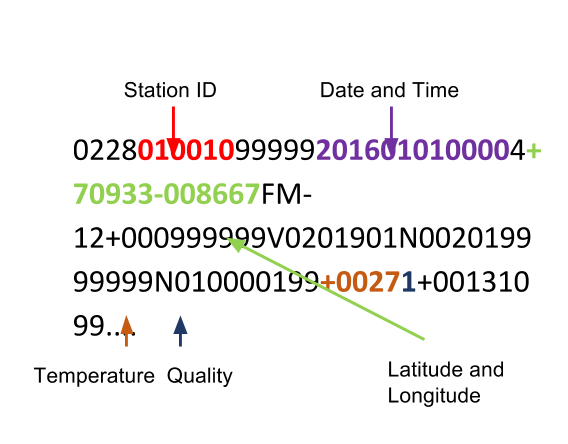
\includegraphics[width=1\linewidth]{data}
\caption{Measurement format}
\label{fig:data}
\end{figure}

Each measurement comes in a form similar to what \ref{fig:data} shows. The information we need for our analysis are: station ID, data and time, coordinates (in latitude and longitude), the temperature value and the quality of the temperature measurement.


\subsection{Temperature data quality}
\label{sec:filter}
Before using the actual temperature data, we filtered it through a custom quality check. Each measurement come with a quality flag set at a different value depending on how reliable the measurement was\cite{noaaDataFormat}.
It is important to use this flag to remove wrong data in the dataset, as reported in the document provided by NOAA that describes the problem inside the dataset \cite{noaaProblems}: ``Various, mostly random errors, are present in the overall dataset, and these are being documented and scheduled for correction. Quality control of the data
(which has already taken place and reflected in the online data) has corrected
well over 99 percent of the errors present in the original data prior to the quality control.''
In particular we accepted all the measurement with the following quality code value:
\begin{itemize}
    \item 0: Passed gross limits check;
    \item 1: Passed all quality control checks;
    \item 4: Passed gross limits check, data originate from an NCEI data source;
    \item 5: Passed all quality control checks, data originate from an NCEI data source;
    \item A: Data value flagged as suspect, but accepted as a good value;
    \item I: Data value not originally in data, but inserted by validator;
    \item M: Manual changes made to value based on information provided by NWS or FAA;
    \item P: Data value not originally flagged as suspect, but replaced by validator;
    \item R: Data value replaced with value computed by NCEI software;
    \item U: Data value replaced with edited value.
\end{itemize}
We opted for a loose policy on the data quality, accepting also values that didn't pass all the quality checks or that were manually or software replaced. We refuted all the codes that stand for erroneous, missing or suspect data that was not manually or automatically checked and replaced by the institution. Furthermore, we applied a bound check for all the values greater than the maximum registered temperature (+61.8 \celsius) and the minimum one (-93.2 \celsius). \\
The data collected can be of two different types depending on the origin: from a fixed weather station or from a mobile one. In the second case, it's possible that the data registered from a mobile station (e.g. on a ship) is reported at a certain position and the following measurement is reported at a different position. Since we didn't distinguish data by time of the day, it's important that the number of measurements from a certain position is approximately the same for different hours. Since this is not guaranteed by moving stations, we decided to filter the measurement obtained from this source. \\

\subsection{Data Sources}
An important aspect we had to consider before proceeding with the analysis is the distribution of weather station on the globe. First we considered the number of stations per year\ref{fig:stations}. Then we analyzed the position of the stations for each year (some notable sample are reported in appendix \ref{App:AppendixA}). 

\begin{figure}[tbh]
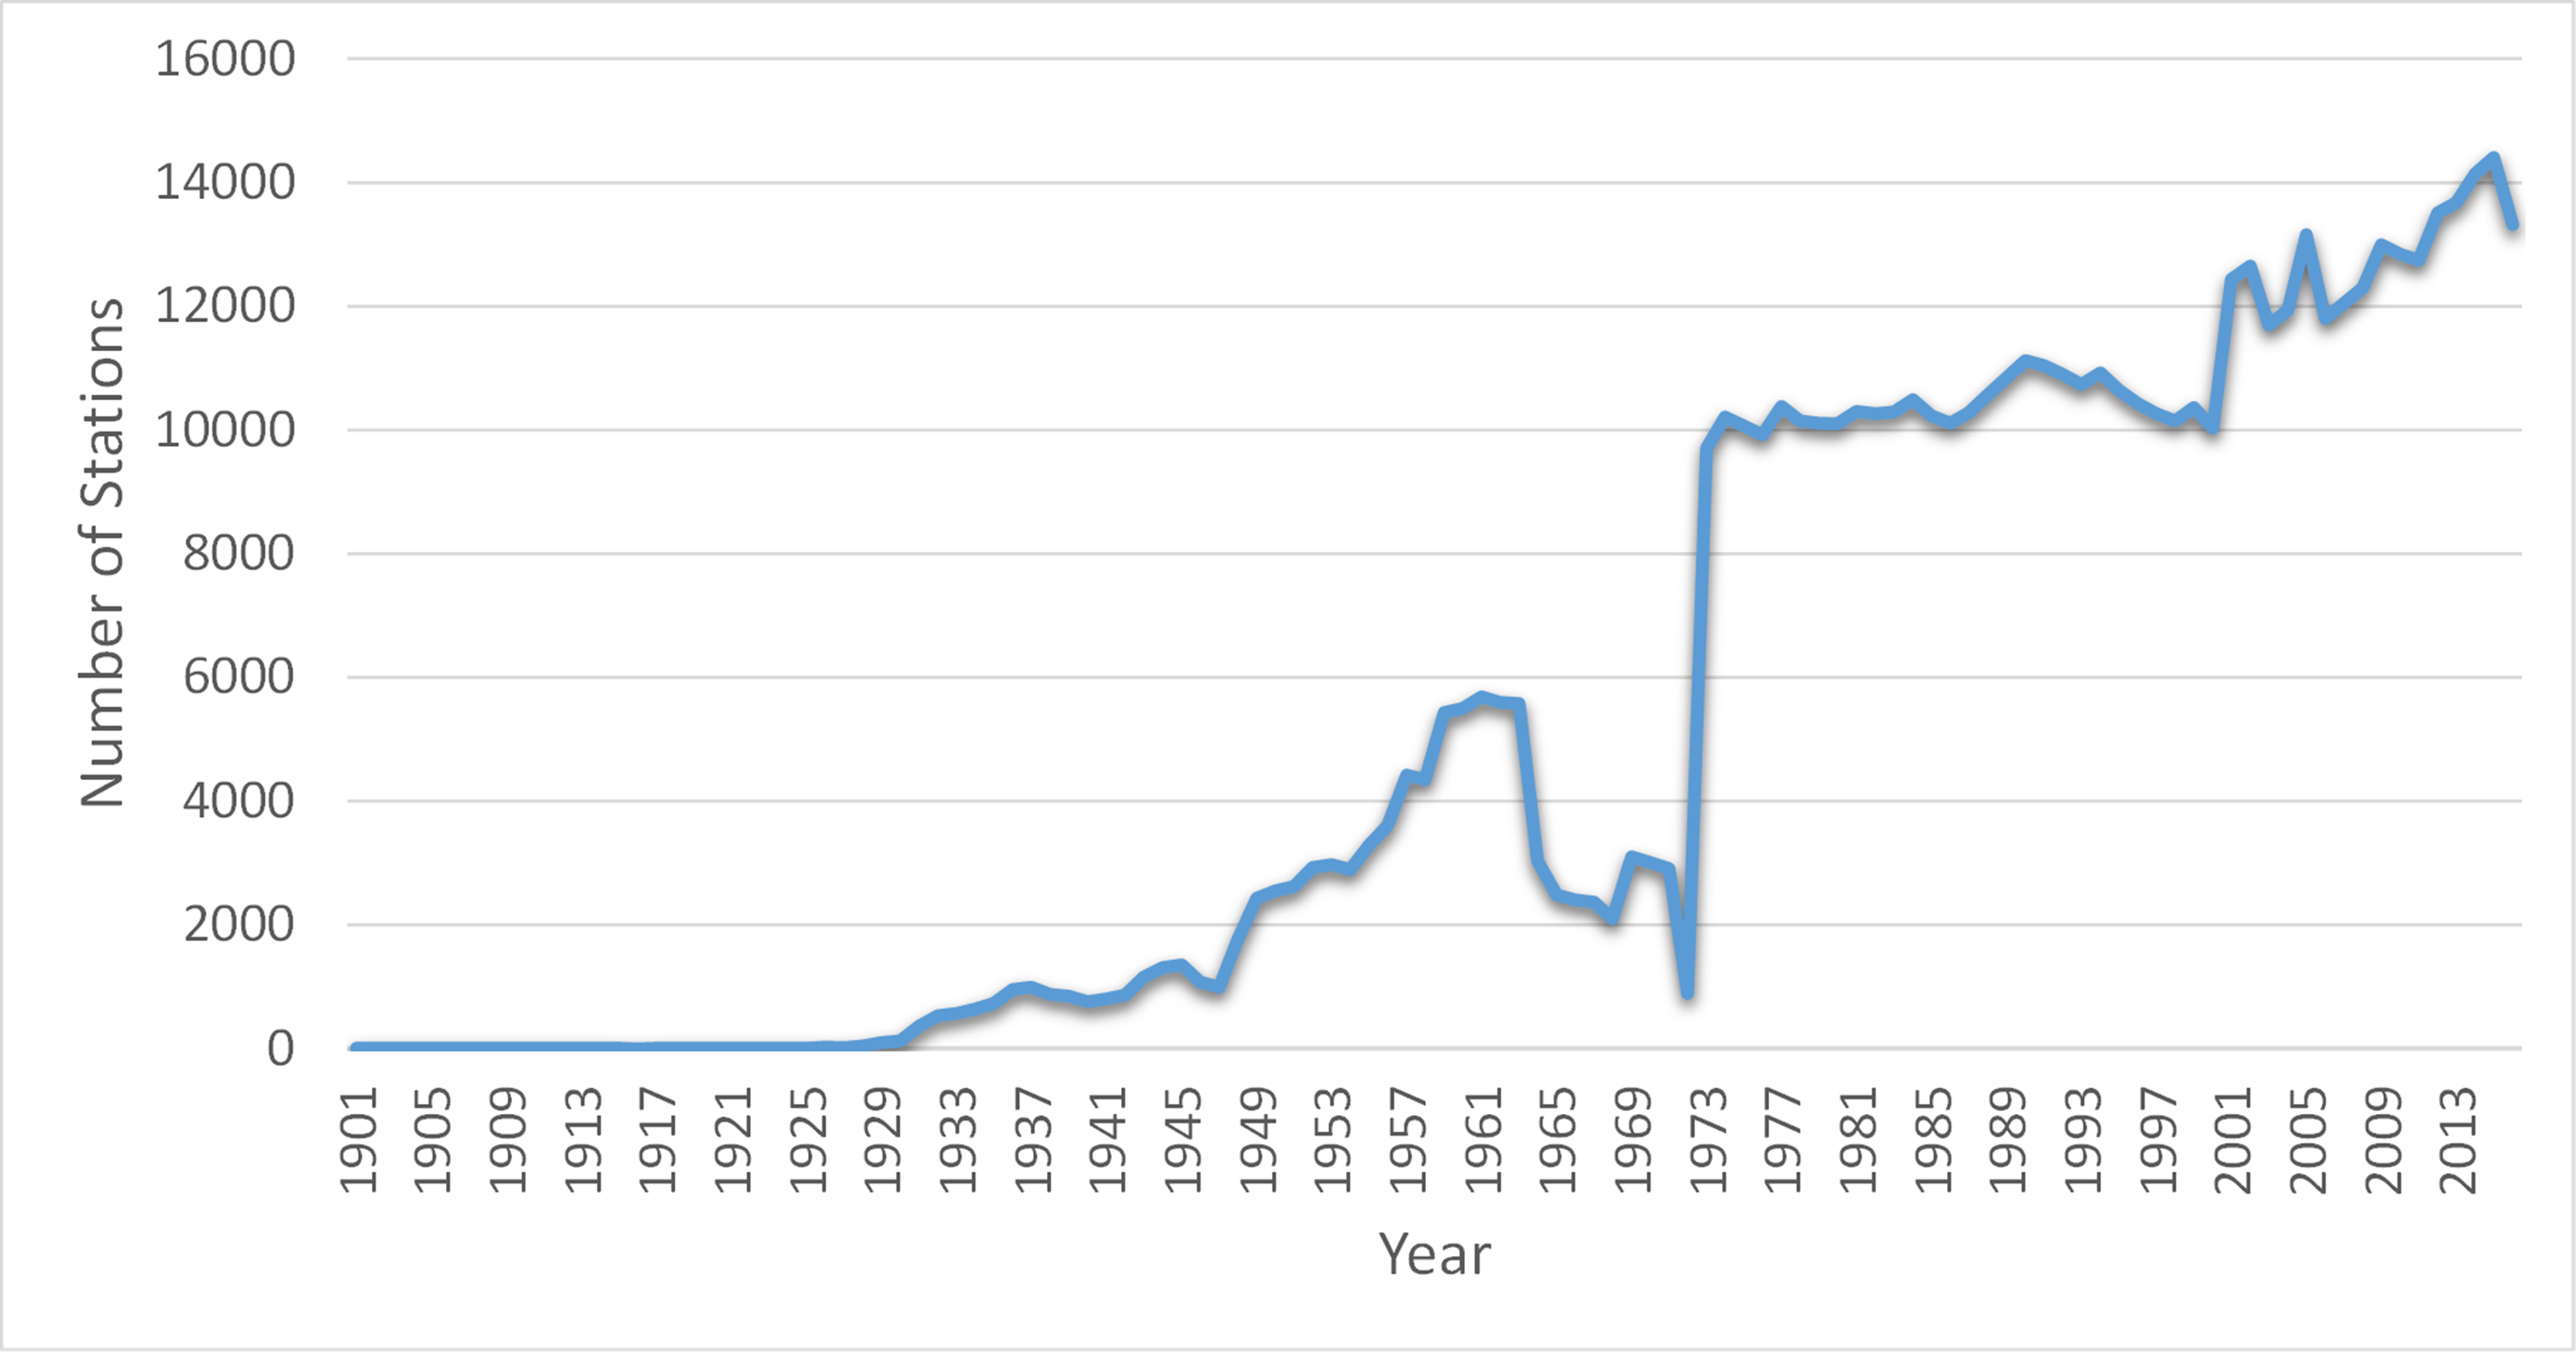
\includegraphics[width=1\linewidth]{stations}
\caption{Number of stations per year}
\label{fig:stations}
\end{figure}

The important things to consider before proceeding with the analysis are:
\begin{itemize}
    \item The stations are not distributed uniformly. In particular, the areas most covered are only a portion of the total surface of the earth and include mostly the land areas (the coverage of the oceans is pretty limited);
    \item There are no guarantees that a station reporting one year will report also the following years;
    \item Although the general trend manifest an increase of the number of stations, this is not always true (e.g. during the late 60's there are less stations reporting);
    \item The years before 1930 show a very low number of stations. We will have take this into account when we evaluate the results for this time frame.
\end{itemize}


\subsection{Data Analysis Environment}
The technological environment we decided to use for this project consist of:
\begin{itemize}
    \item \textbf{HDFS}\cite{hadoop}: a distributed file system that allows the developers to store and retrieve large quantity of data between multiple machines as if it was a single one;
    \item \textbf{Spark}\cite{spark}: programming framework to develop applications for large scale data processing on horizontally scalable clusters.
\end{itemize}

\textbf{HDFS}

\begin{figure}[tbh]
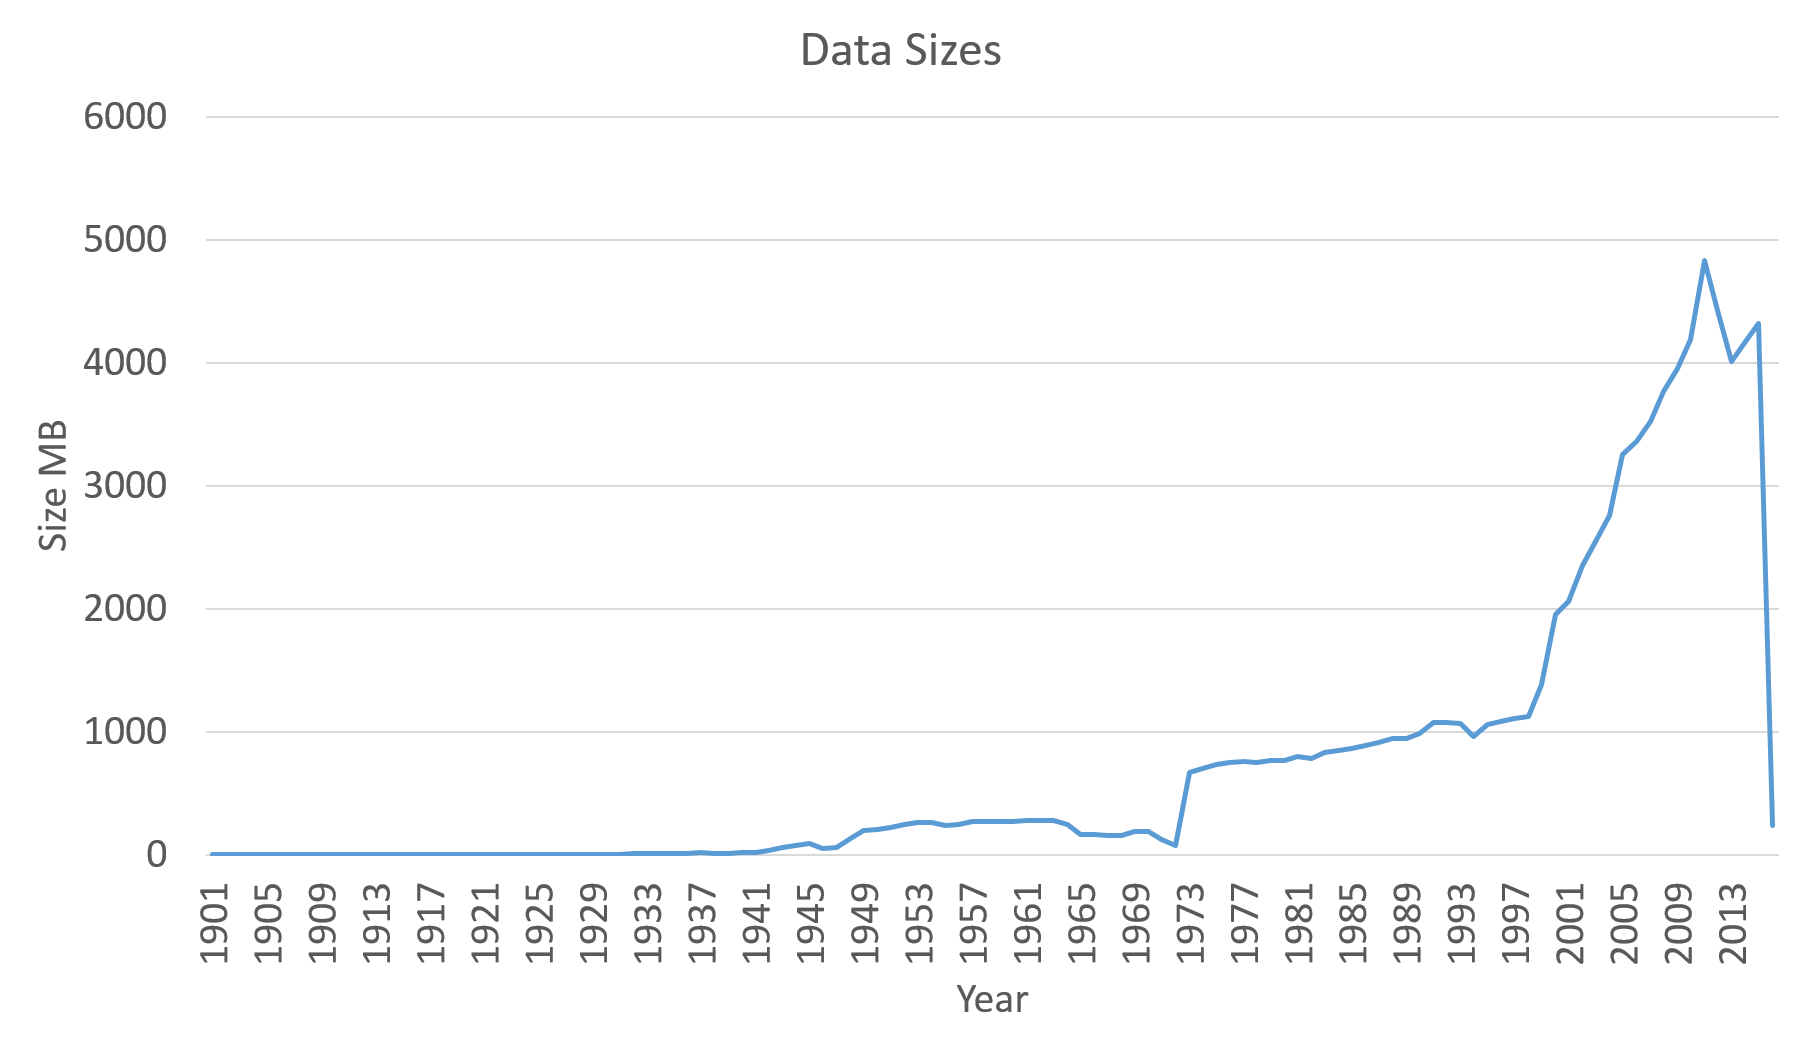
\includegraphics[width=1\linewidth]{dataSize}
\caption{Size of the data per year.}
\label{fig:dataSize}
\end{figure}

The data stored in the distributed file system is grouped in folders by year. As shown in figure \ref{fig:dataSize} the size of the data to analyze is very different between the years. Inside each folder, there is a file for each station that reported measurements. HDFS is not very efficient when working with many small files\cite{zhang2012improving}, as in our case. The solution we opted to use is to merge the small files in bigger files that have the same size as Hadoop's default block size. To merge the files we used filecrush\cite{filecrush}. This tool merges small files, located inside an HDFS instance, into bigger files with the size of a multiplier of an HDFS block. We have run this tool one time for each folder of the data. The number of total files was reduced by an order of magnitude of $10^2$.\\

\textbf{Spark}
The choice of this technology is motivated by size of the data and the type of the analysis we want to execute. First, Spark is more efficient than Hadoop's own MapReduce\cite{dean2008mapreduce} implementation when the data used can fit in memory. Since our approach is to analyze one or a few years at a time, we calculated that the size of the data is small enough to stay in memory for our purposes. \\
The second advantage is that we would like to make multiple transformations to the data and Spark allows to easily cache the intermediate results to be reused efficiently. In this way, there is no need continuously store the results and load them to be reused for the next MapReduce operation. One example is calculating the large region averages, for which we make use of the intermediate results of the worldwide regions (each one of equal size) analysis\ref{fig:analysis}. The caching feature is used multiple times throughout the execution and drastically improve the performance. \\

\textbf{SURFsara Hadoop cluster}
All the computation are executed on the SURFsara Hadoop cluster \cite{surfsara}. The cluster is one of the largest Hadoop clusters for scientific research in the Netherlands. It is composed of 170 data/compute nodes with a total 1370 CPU-cores for parallel processing. The system has also a distributed file system that has a capacity of 2.3 PB. The cluster is shared and used by different users that needs an HPC infrastructure for their research.   

\FloatBarrier

\section{Experiments}
\label{sec:exp}
We performed two main type of analysis: a five year span analysis that considers all the measurement reported by stations near each other in five years, and an analysis on large earth regions on a yearly basis. \\

\begin{figure}[tbh]
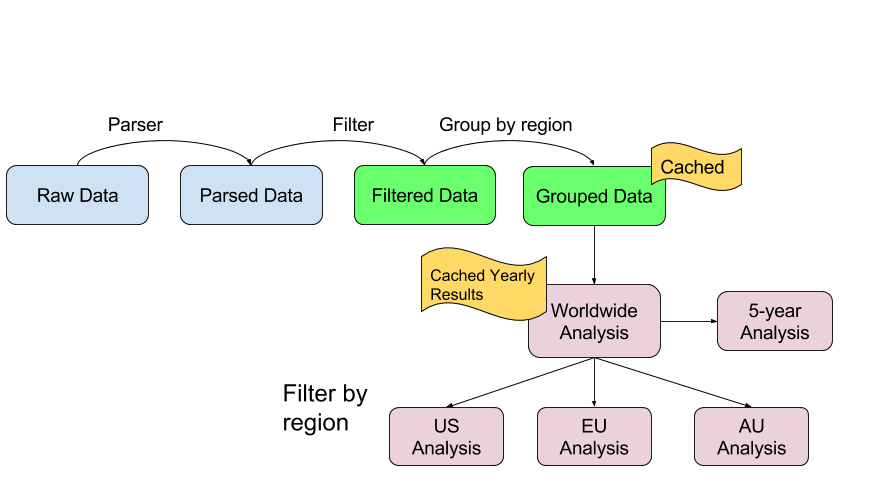
\includegraphics[width=1\linewidth]{analysis}
\caption{Analysis scheme}
\label{fig:analysis}
\end{figure}


The basic steps that both analysis perform are:
\begin{enumerate}
    \item Load data in memory;
    \item Parse the raw data to obtain an list of StationData (a type that represent a measurement);
    \item Filter data following the scheme indicated in \ref{sec:filter};
    \item Group the measurements in regions;
    \item Execute yearly analysis;
    \item Execute 5-year analysis starting from the results of the yearly analysis;
    \item Save results;
\end{enumerate}

\subsection{Regional five year period analysis}
The aim of this analysis is to calculate the temperature statistics (mean, maximum, minimum and standard deviation) on every area of the earth for which we have data. After that we can compare the situation for the same areas in different time frames and show it with a world map view (as shown in \ref{sec:map}). \\
The first problem is that while the regions we want to compare are the same size and uniformly distributed around the earth, the stations are not. Furthermore a lot of stations are added and removed during the flow of the years, this means that the data of a new station couldn't be compared with any data of the previous years even if in the previous years there was a station very close to the new added station. So we defined regions of size 1\degree latitude and 1\degree longitude. This is approximately the area covered by the region of Holland in the Netherlands. Then we assigned each measurement (for each one there is the coordinates reported) to a region. \\
Our analysis proceeded by loading five consecutive years of measurements at a time, group them in small regions and, for each region, calculate the arithmetic mean, the minimum, the maximum temperature and the standard deviation. This was done for all years from 1901 to 2015 (the year 2016 was excluded from the analysis due to incomplete data).\\
\subsubsection{Median}
Another value we wanted to extract from the datasets is the median. We implemented the code to calculate it, but we didn't have enough time to test it and obtain the results for all the datasets. The problem with calculating the median is that it is not a commutative and associative operation (the median of medians is not the median of the entire group). This means that there is no easy way to use the reduce function to combine results computed in different machines in a distributed way. The simple way to calculate the median is to sort the desired data and look at the value in the middle. The problem with this solution is that it's not scalable. Indeed, applied to datasets in the order of GB in sizes this operation is very slow. Work has been done by various researchers to tackle this kind of problems and improve the efficiency of non associative operations (\cite{liu2009computing}).


\subsection{Zonal Analysis}
In this type of analysis we focused on some particular large areas of on the earth. We selected the regions that for which we have more and better distributed data available. The selected regions are:
\begin{itemize}
    \item United States: from coordinate N\ang{50;;} W\ang{128;;} to N\ang{24;;} W\ang{65;;};
    \item Europe: from coordinate N\ang{71;;} W\ang{11;;} to N\ang{35;;} E\ang{41;;};
    \item Australia: from coordinate S\ang{9;;} E\ang{111;;} to S\ang{44;;} E\ang{156;;};
\end{itemize}
For each region we calculated minimum, maximum, average and standard deviation of every year until 2015. The year range is chosen based on the availability of data. 

\begin{figure}[tbh]
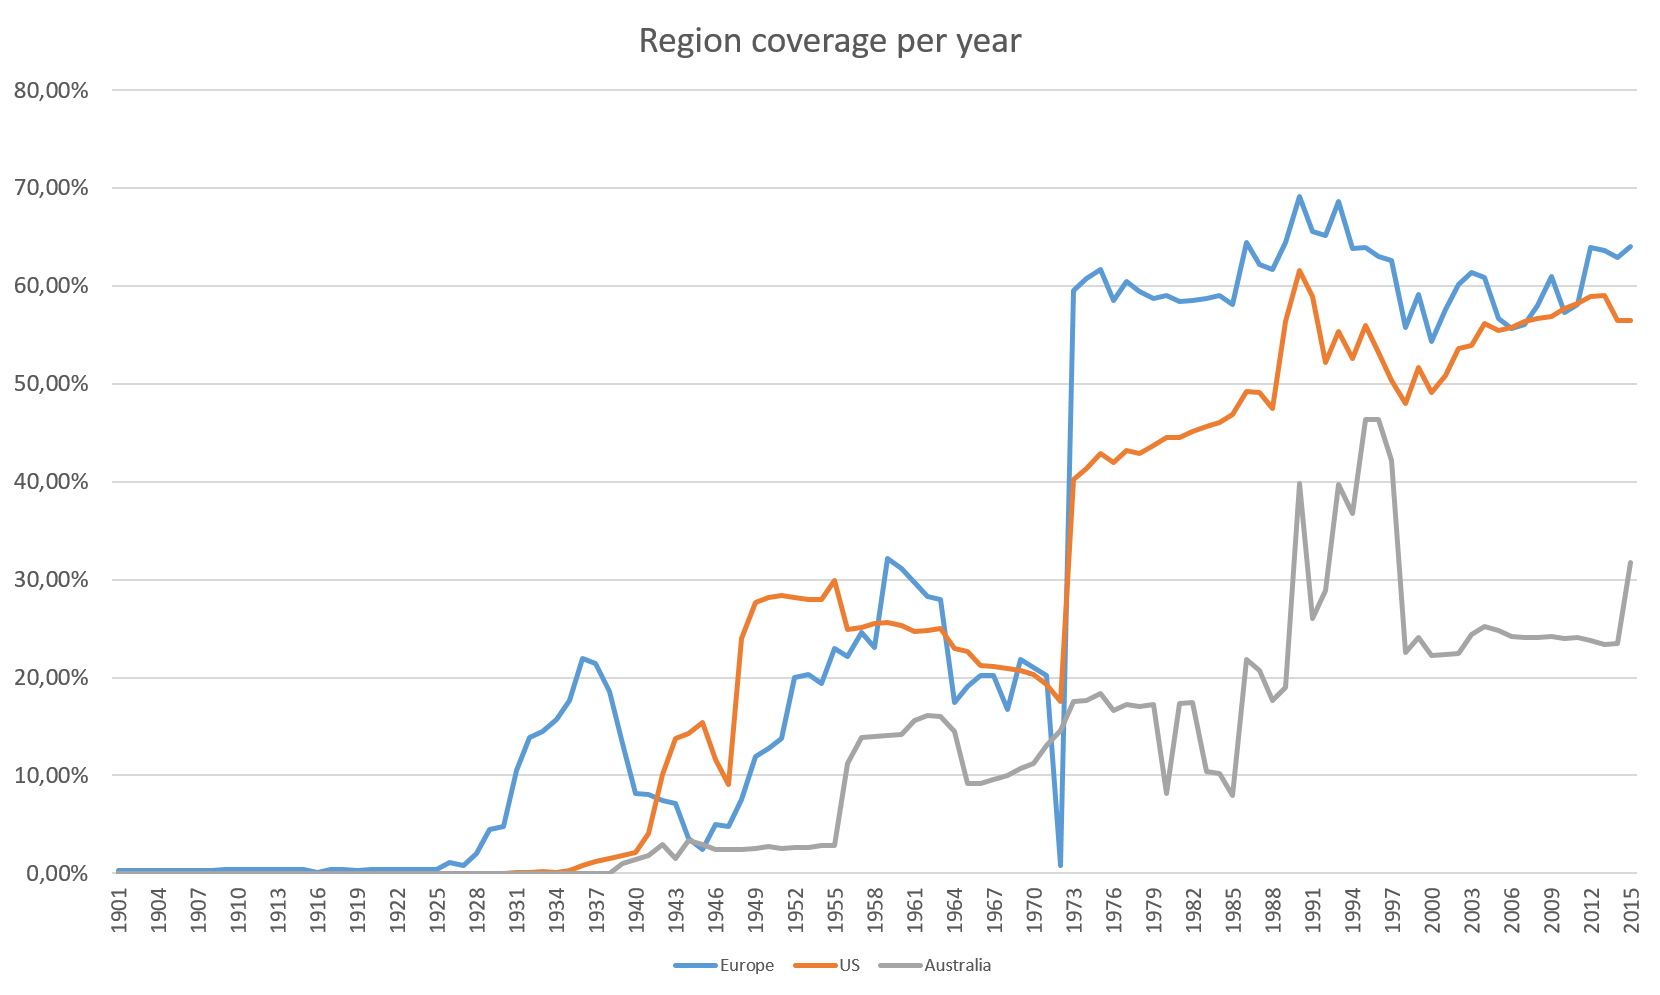
\includegraphics[width=1\linewidth]{stationsRegion}
\caption{Percentage of regions covered by at least one station per region.}
\label{fig:stationsRegion}
\end{figure}

The chart in figure \ref{fig:stationsRegion} shows the surface coverage of the selected regions for each year from the data we analyzed. As we can see, we don't have data from every part of the regions, with Europe and US the more covered ones (with peaks of 70\% and 60\%). The are two main reason behind this:
\begin{itemize}
    \item In the chart we took into account the number of regions for which we have data on the total amount of regions in the area. With a different selection of region size we could increase or decrease the total coverage (at the expense of precision).
    \item There may be areas in the regions where it's more difficult to have a uniform stations coverage because of geomorphological reasons. For instance, there are far less regions covered in the middle part of Australia due to its desert climate, which makes it more difficult to install, maintain and monitor the stations.
\end{itemize}


\subsection{Results format}
The results computed by the program we developed with Spark are stored in HDFS with the CSV format. The results are stored in multiple HDFS folders, one per each year. Inside each folder there are multiple CSV files with portions of the yearly results. To collect the results from HDFS and compact them we developed a script that merges the files in each folder in two CSV files per each year. One file contains the minimum and the maximum temperature for each latitude and longitude quadrant. The other file contains the value of the average and of the standard deviation of the temperature.
The script, in addition to the two CSV files, creates two JSON files with the same information. Those files will simplify the parsing of the data in the graphical user interface that is developed with javascript. 
\\ The results of the zonal analysis are stored in one single CSV file per each zone containing one row per each year. With this format it is easy to create some charts about the change of the temperature for that zone during the years.



\FloatBarrier

\section{Results}
\label{sec:res}
In this section we report the results obtained from the analysis described in section \ref{sec:exp}. 

\subsection{Interactive map}
\label{sec:map}
The first tool we worked on is a dynamic map that allows to visualize the difference between temperature values (average, maximum, minimum and standard deviation) between two datasets. Each dataset is created from the analysis one described in section \ref{sec:exp} and are composed of the aggregated results of the five yearly analysis in which we divided the surface in small regions of 1\degree latitude and 1\degree longitude. \\
We used the map provided by Google\cite{maps}. We created a custom heatmap that shows on each region of the map different colors to show an increase or decrease for a particular value in that region (shades of blue for reduction and red for a gain). The interface can be seen in figure \ref{fig:interface}

\begin{figure}[tbh]
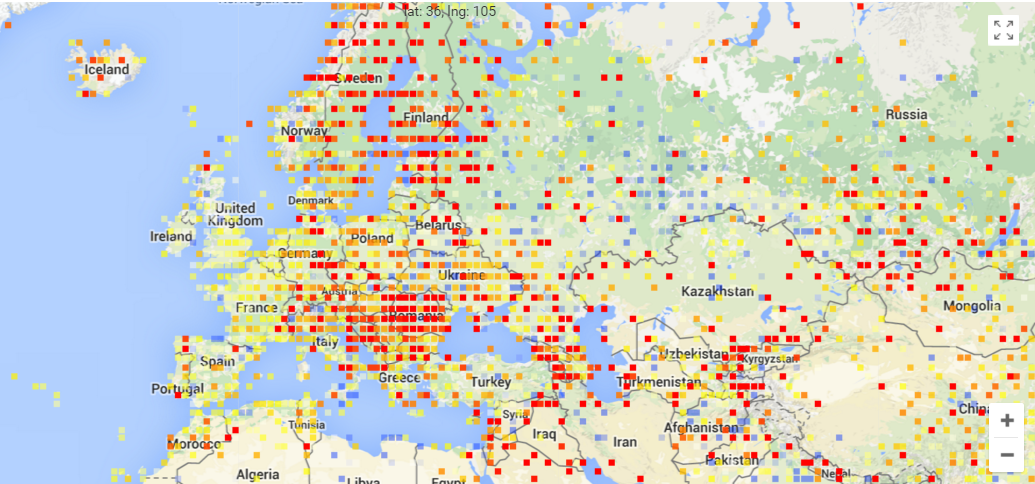
\includegraphics[width=1\linewidth]{interface}
\caption{Interactive map interface example}
\label{fig:interface}
\end{figure}

In the graphic interface there is the possibility to select the two set of five-year results to compare. The heatmap shows a colored square in a latitude and longitude quadrant if it's present a data for that quadrant in both the two sets of results. Till the period 1921-1925 there are few data in the results, with consequently few colored squares in the map. In the interface there is also the possibility to change the temperature metric that is used to compare the two set of results.\\
One problem of the interface is that the colored squares used in the map should change their height depending on the latitude value where they are positioned because the map projection isn't equiareal. The consequence in the heatmap visualization is that there is some empty space between the squares of a certain latitude value and the squares with the value of the latitude increased or decreased by one. This aspect makes the heatmap looks like as it is missing some data for certain latitude when instead the data are present, just the squares should be rectangles with a bigger height value.\\

By using the interactive map it is possible to notice an increase of the global temperature in the years from 1975 to the current years. In figure \ref{img:increaseMap} it is possible to see an example of increase of the average temperature between the two interval 1976/1980 to 2011/2015 in Europe and in Asia. The red colors are dominant in all the figure. Showing an increase of at least 2.5 degrees for all the regions that have a red square over them.
In figure \ref{img:increaseGlobal} it is possible to see how the minimum temperature is increased for the same two intervals of years in the majority of regions of the world.

\begin{figure}[tbh]
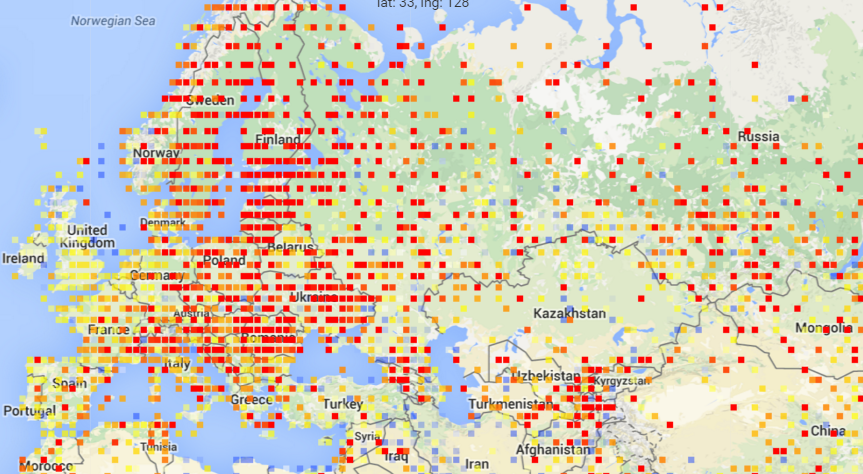
\includegraphics[width=1\linewidth]{increaseEurope}
\caption{Map that shows the increase of the average temperature in Europe and in Asia between 1976 and 2015.}
\label{img:increaseMap}
\end{figure}

\begin{figure}[tbh]
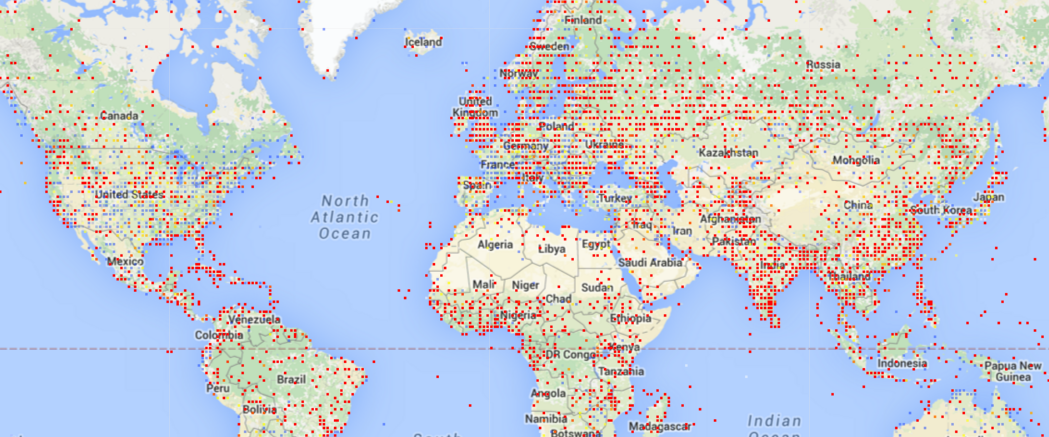
\includegraphics[width=1\linewidth]{increaseGlobal}
\caption{Map that shows the increase of the minimum temperature globally between 1976 and 2015.}
\label{img:increaseGlobal}
\end{figure}

\subsection{Zonal Analysis}
In this section we report the results of the regional analysis done for: Europe, United States and Australia.

\begin{figure}[tbh]
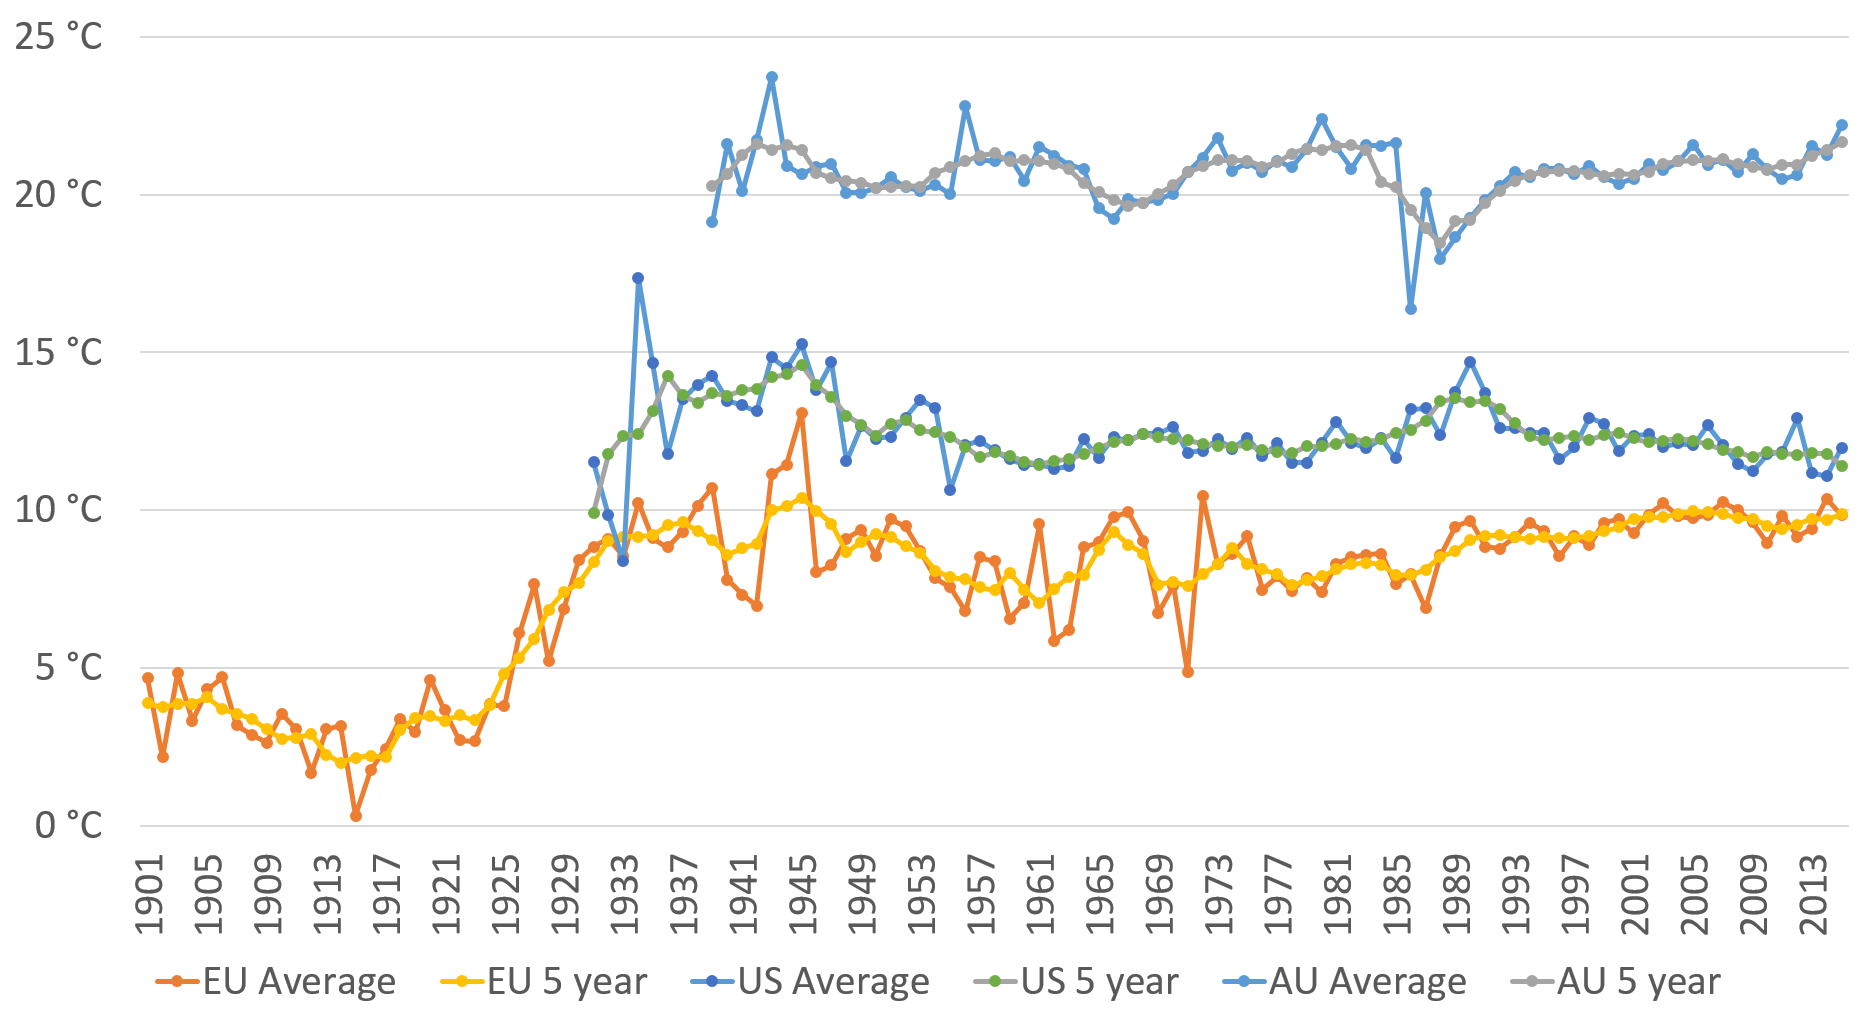
\includegraphics[width=1\linewidth]{averageRegions}
\caption{Average and 5-year average for three different regions.}
\label{fig:averageRegions}
\end{figure}

In figure \ref{fig:averageRegions} we show the evolution of both the average and the 5-year average for the three region we considered. The first thing to consider is that the in the earlier years we have less data available. For instance in Europe, we have data mostly from stations in Finland for the period 1901-1930. This explain two anomalies in the chart:
\begin{itemize}
    \item A sudden change in the average temperature between two time frames (the sudden increase in the average temperature for Europe is caused by the presence of new stations in warmer areas);
    \item The variance of annual temperatures is more evident in the years with less data and stabilizes for all three regions from the last decades of the century.
\end{itemize}

\subsubsection{Temperature Anomalies}
In figure \ref{fig:UsAnomalies}, \ref{fig:EuAnomalies} and \ref{fig:AuAnomalies} we used the same method described by Hansen (\cite{hansen1999giss}) to calculate the temperature anomalies for each dataset. We first calculated a total average value for each region for the time frame examined. Then we calculated the difference between the yearly average values and the total obtained. In this way it's easier to spot extremely hot or cold years and a general temperature trend. 


\begin{figure}[tbh]
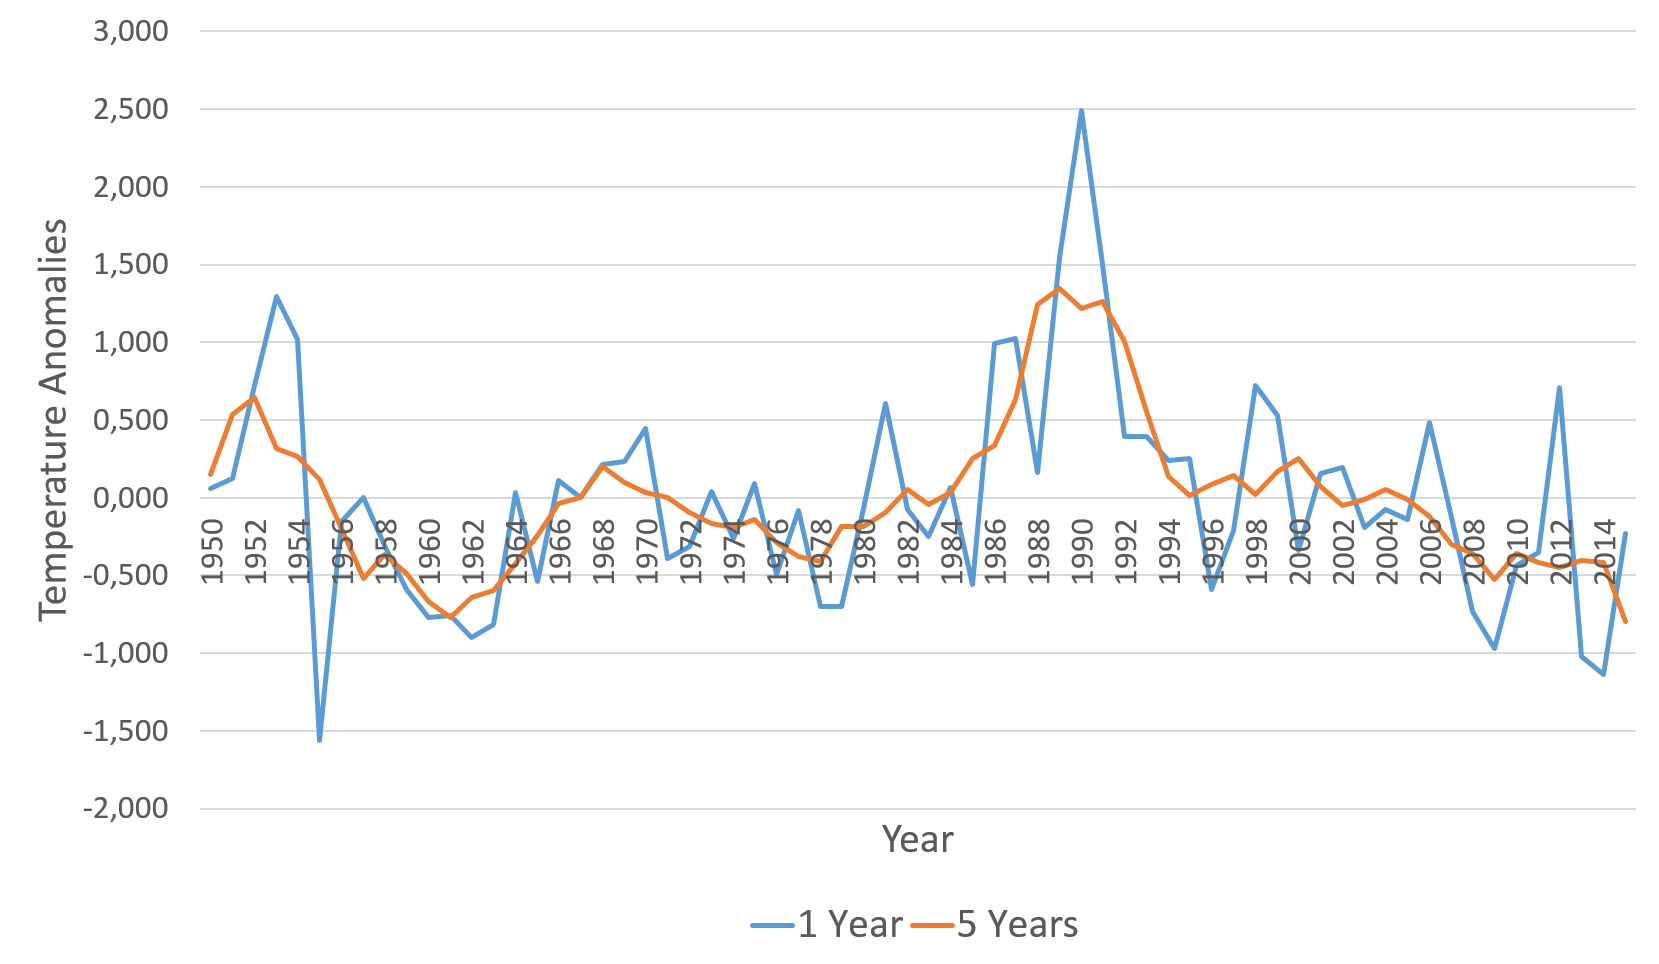
\includegraphics[width=1\linewidth]{UsAnomalies}
\caption{Average and 5-year average for three different regions.}
\label{fig:UsAnomalies}
\end{figure}

From the US chart (\ref{fig:UsAnomalies}) the interesting thing to notice is a slightly warming trend between the 60s and 70s and an opposite one for the last thirty years. This goes in accordance with the observation made by other researchers\cite{hansen2006global}. The main suspect for this phenomenon is thought to be the hurricane El Nino that hit the US in 1998.

\begin{figure}[tbh]
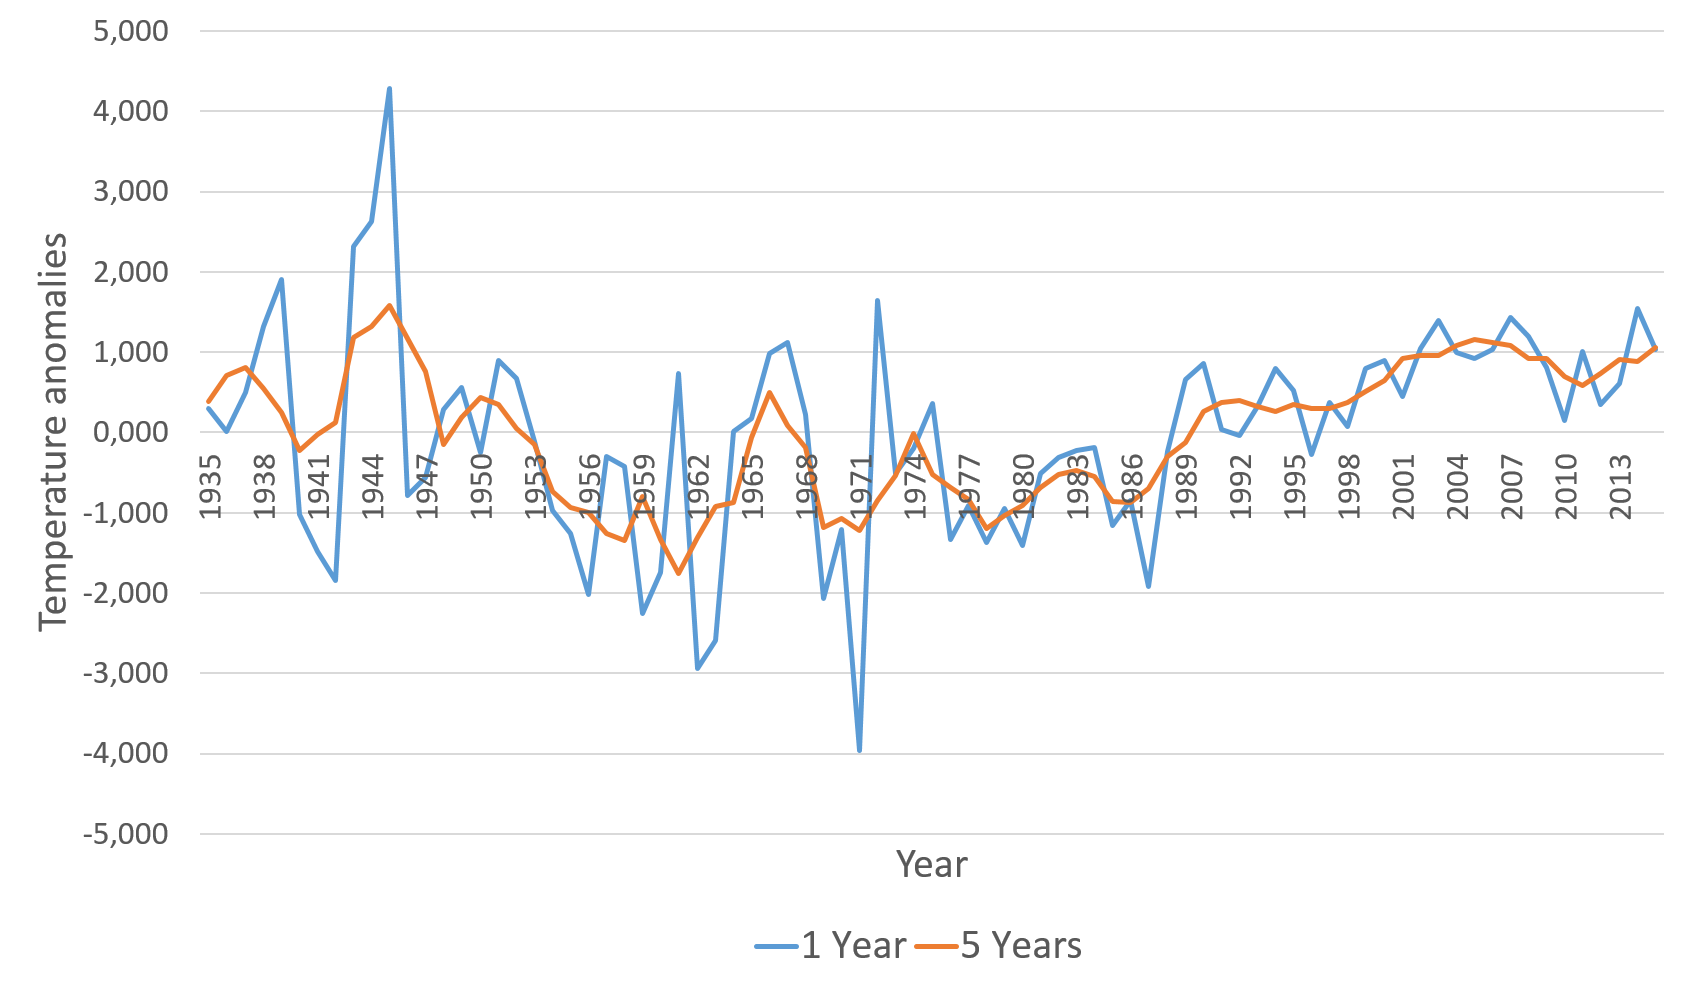
\includegraphics[width=1\linewidth]{EuAnomalies}
\caption{Average and 5-year average for three different regions.}
\label{fig:EuAnomalies}
\end{figure}

The EU chart shows, starting from the late 70s, a pretty clear trend of temperature increase. Interesting also to note the high average temperatures in the period 1940-1945, during WW2. We leave to the reader to use the interactive map we created to correlate the data sources distribution and the temperature levels.

\begin{figure}[tbh]
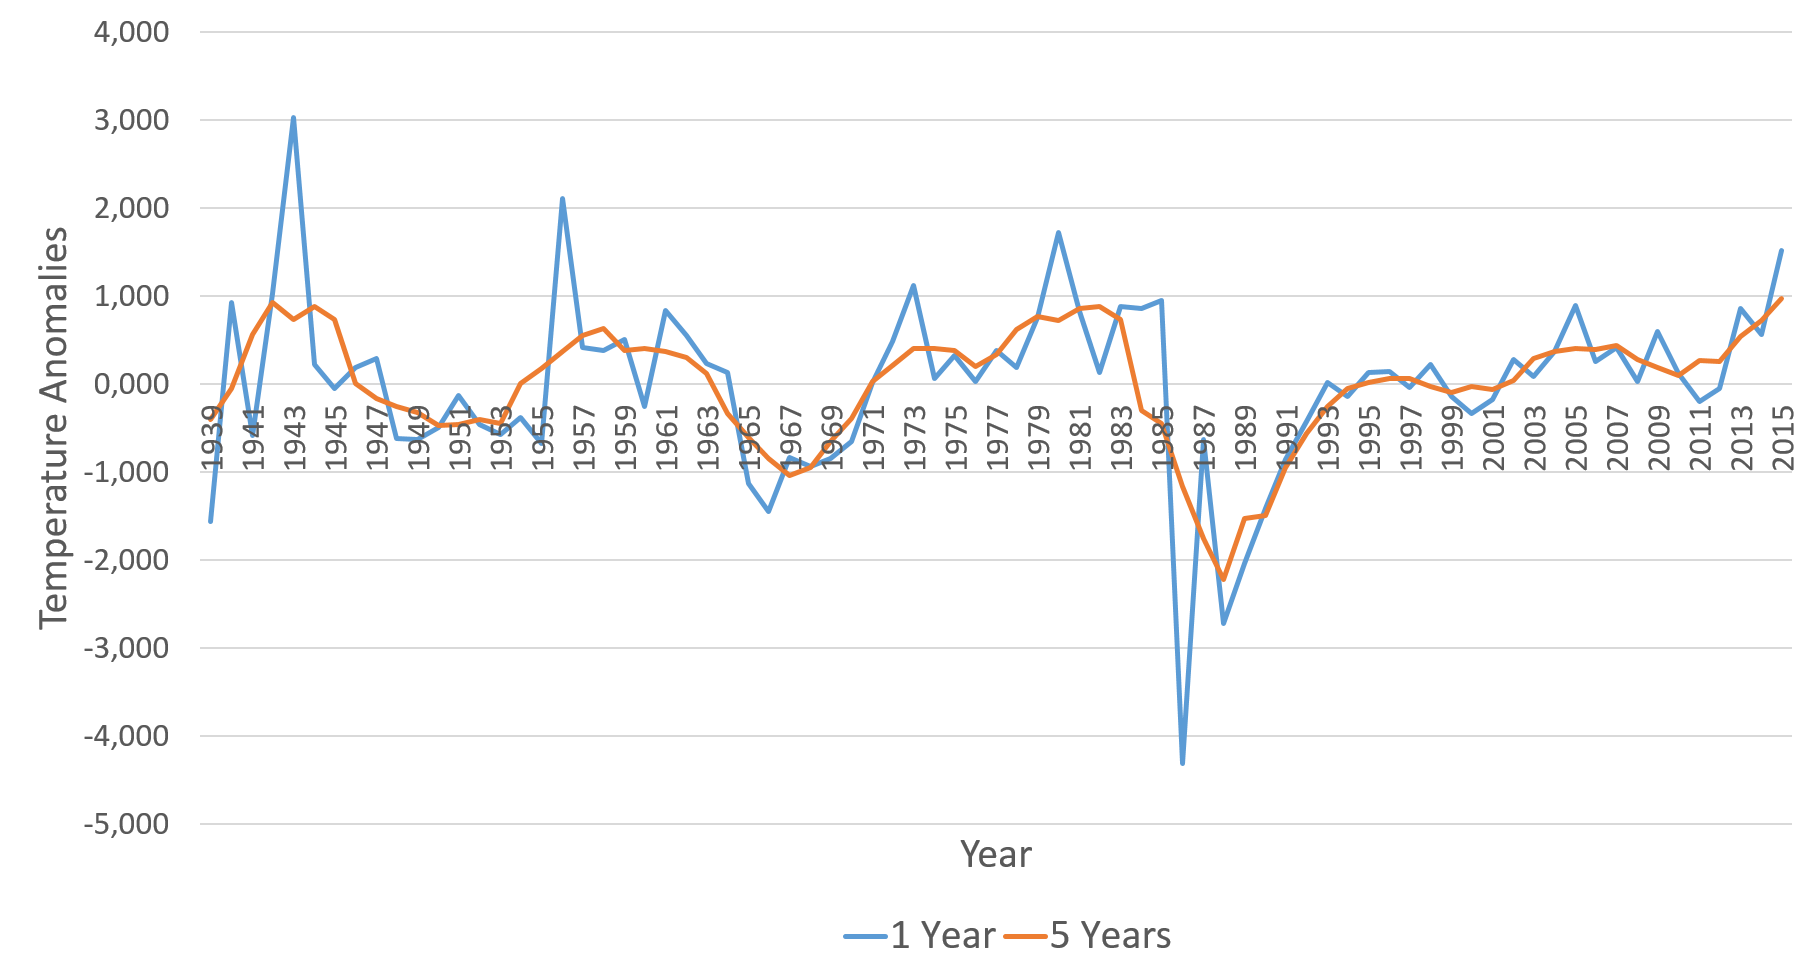
\includegraphics[width=1\linewidth]{AuAnomalies}
\caption{Average and 5-year average for three different regions.}
\label{fig:AuAnomalies}
\end{figure}

For the Australia data the most interesting fact we notice is a sudden plunge in the temperature during the 80s. This can be explained by looking at the stations number chart for that region, that manifest a decrease for the same period of time. As for the European situation, we can see a slight increase in the average temperature, that is confirmed by the results of other studies, that shows an increase of the average temperature for the Australian continent of about 0.8\degree. 

\subsubsection{Standard Deviation analysis}
\begin{figure}[tbh]
\label{fig:stdev}
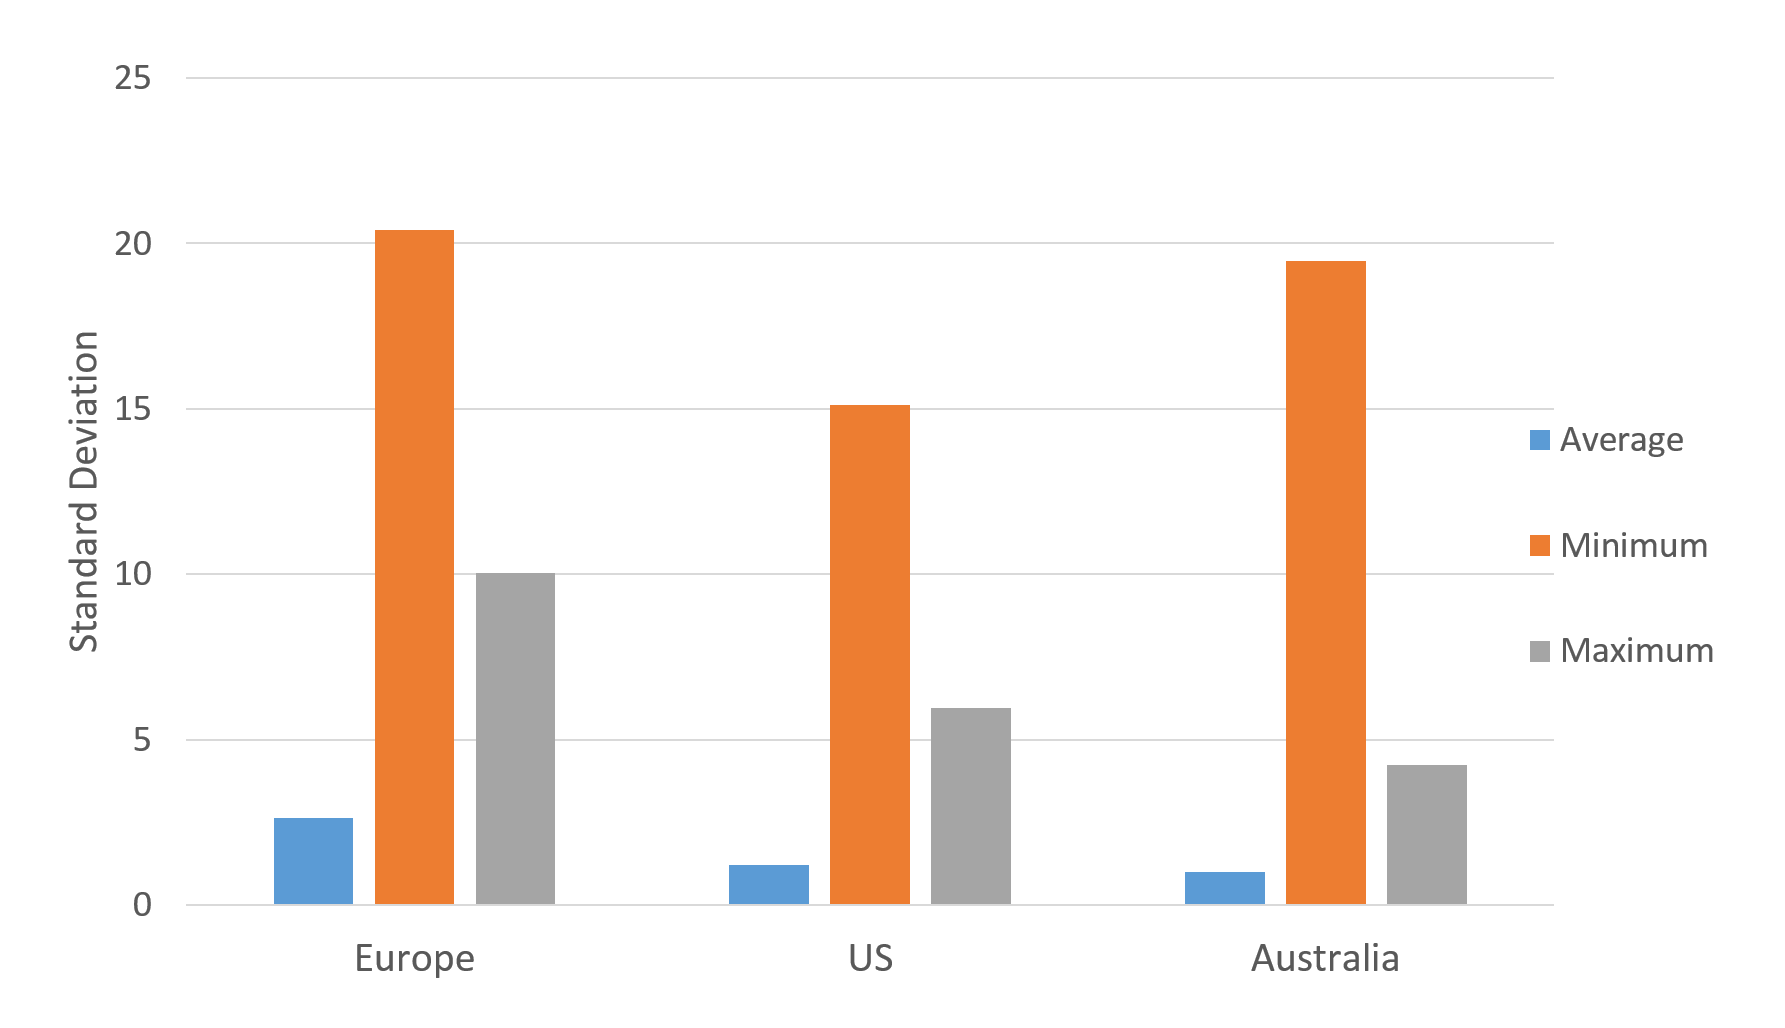
\includegraphics[width=1\linewidth]{stdev}
\caption{Standard deviation for Average, Minimum and Maximum values per region.}
\end{figure}
In figure \ref{fig:stdev} we plotted the value of the standard deviation per statistics and per region. It's clear that the values of maximum and minimum have larger fluctuation than the average. This may be caused by one or a few erroneous data report caused by environmental accidents. Interesting to note that the minimum value have a way larger standard deviation that the maximum. By correlating this with the stations distribution we came to the conclusion that this is caused by the installation of new stations in more remote and difficult to access regions (e.g. Arctic ocean and mountain regions). \\
Moreover, the minimum standard deviation for the Australian region was suspect, because the lowest temperature registered for the region is -23.4\degree C\cite{ausTemp}, so it's difficult to expect a standard deviation similar to that of the European region or even higher than that of the American one. After analyzing the data we found out erroneous data coming from the south east region of Australia reporting temperature of around -70\degree C.

\FloatBarrier

\section{Conclusions}
\label{sec:con}
Before answering the question we asked earlier we will take a brief general overview of the characteristics of this project. One of the main problem we encountered is the limited (if not absence) of documentation describing the data. Especially for the older datasets we had to directly analyze the data to know the origin (region on earth) or the time coverage (day/night reports, coverage of all months). Moreover, we had to take into account during the analysis and the result discussion the anomalies we discovered in the station number charts (\ref{App:AppendixA}). Without a uniform and well formed source it's more difficult to extract reliable statistics.\\
We are overall satisfied with the performance of the program developed with Spark for analyzing the data. The program is able to analyze the entire dataset in approximately 8 hours. The program is also scalable to the data size. Future data in the next years will probably grow in dimensions, Spark can automatically handle new resources available in the cluster if there is the need. Furthermore the structure of the program allows also to manage the growth of the data by computing some intermediate results on the yearly data. The five year analysis is performed only on these intermediate results that are way smaller than the initial data. This feature removes the need to join all the data of the five years.\\
Other two aspect that improve the performance are the step we performed to group the big amount of files, and the caching of the data after the operations of parsing, filtering and grouping. The first improvement makes HDFS to be faster because it performs much better with a smaller amount of bigger files. The second improvement allows to compute different analysis on the same data without redoing some computation that are needed in the different types of analysis.\\

For what concerns the metrics used for analyzing the data, the average temperature is the most useful metric. It shows clearly the increase of the temperature in different periods. Also, it's stable even if some particular events happen in short periods of the year. Minimum and maximum temperature are more susceptible to those events and indeed they show less clearly the increase of the temperature in the periods where the average metric reveals the increase. The standard deviation metric is useful to understand if there are errors in the data or if the data are not uniformly distributed (e.g. when the distributions of the stations is changed during the five year of the grouped results then the standard deviation results higher).

\subsection{Global Warming remarks}
From the worldwide analysis and using the interactive map, it appears that a clear temperature increase is in place around the world. Moreover, we notice this phenomenon occurring even considering specific large regions of earth where two out of three show a clear temperature increase trend for the last 30 years, which is in accordance with the data reported by independent researches\cite{hansen2006global}. \\
What we miss in the picture is the data coming from most of the oceanic areas and in general ocean temperatures. The only sources we had that covered large part of the oceans were coming from mobile stations installed on ships. The problem with this data was dual: many times we had the results (average, minimum and maximum) for a region constituted by only one station report. In the end we excluded these from the analysis because they skewed the results in an unpredictable way.


\subsection{Future Improvements}
Due to the limited amount of time available, there are many improvements to the analysis and other research path to discover for a better understanding of the dataset and the global warming phenomenon. \\
To improve the data quality we could divide the temperature data by time of day. We assumed that all the station have a similar behavior (they collect temperature samples every fixed amount of time). Without this assumption the average temperature result could lean towards lower or higher temperatures depending on which the hours for which we have more data.\\
Another interesting analysis that can be performed is dividing the regions by latitude bands. We expect that regions in the same latitude have lower differences in temperature so we could expect a more stable average temperature and less fluctuations in minimum/maximum values. The same reasoning can be done for seasons. In particular it would be particularly interesting to see the temperature changes by season for a fixed region and compare the season analysis (e.g. see if all seasons show the same curve or not).\\ 
An intriguing data source we had available but didn't use yet is the Arctic ice surface coverage. Since this is directly correlated with global temperature and is also one of the most monitored metric in recent years (due to its effects on the ecosystem), we think it can help in strengthening our conclusions. We didn't investigate further this path because our understanding of the data sources was limited and required more time than we expected to interpret correctly the data.

\clearpage

\appendix
\section{Stations distribution} \label{App:AppendixA}
Here is an overview of the stations for some selected years. We decided to show only years in which the number and position of the stations is significantly different than in the previous or following years.

\begin{figure}[tbh]

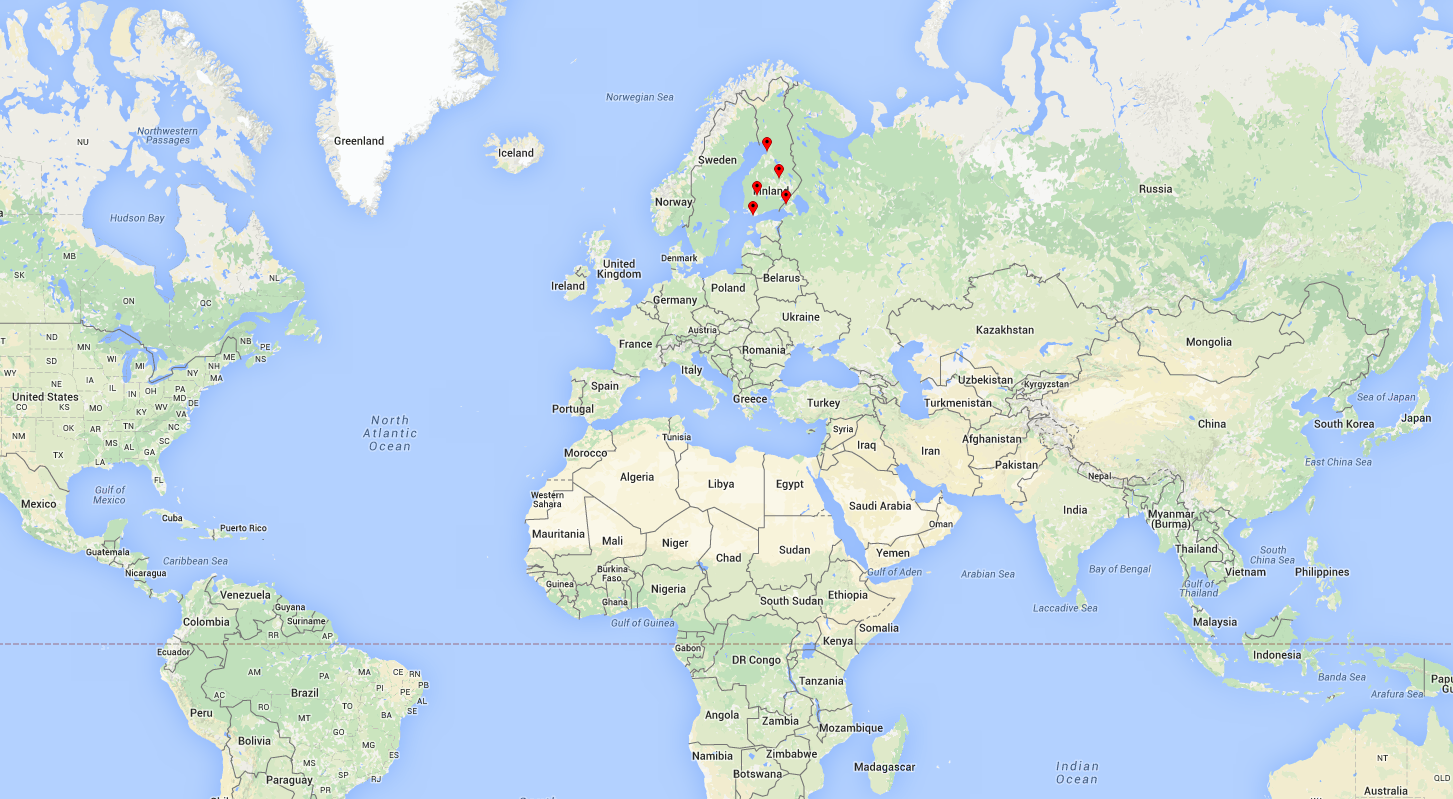
\includegraphics[width=1\linewidth]{stations1907}
\caption{Weather stations used in 1907. In the first years we only have measurements coming from stations in Finland}
\label{fig:stations1907}
\end{figure}

\begin{figure}[tbh]
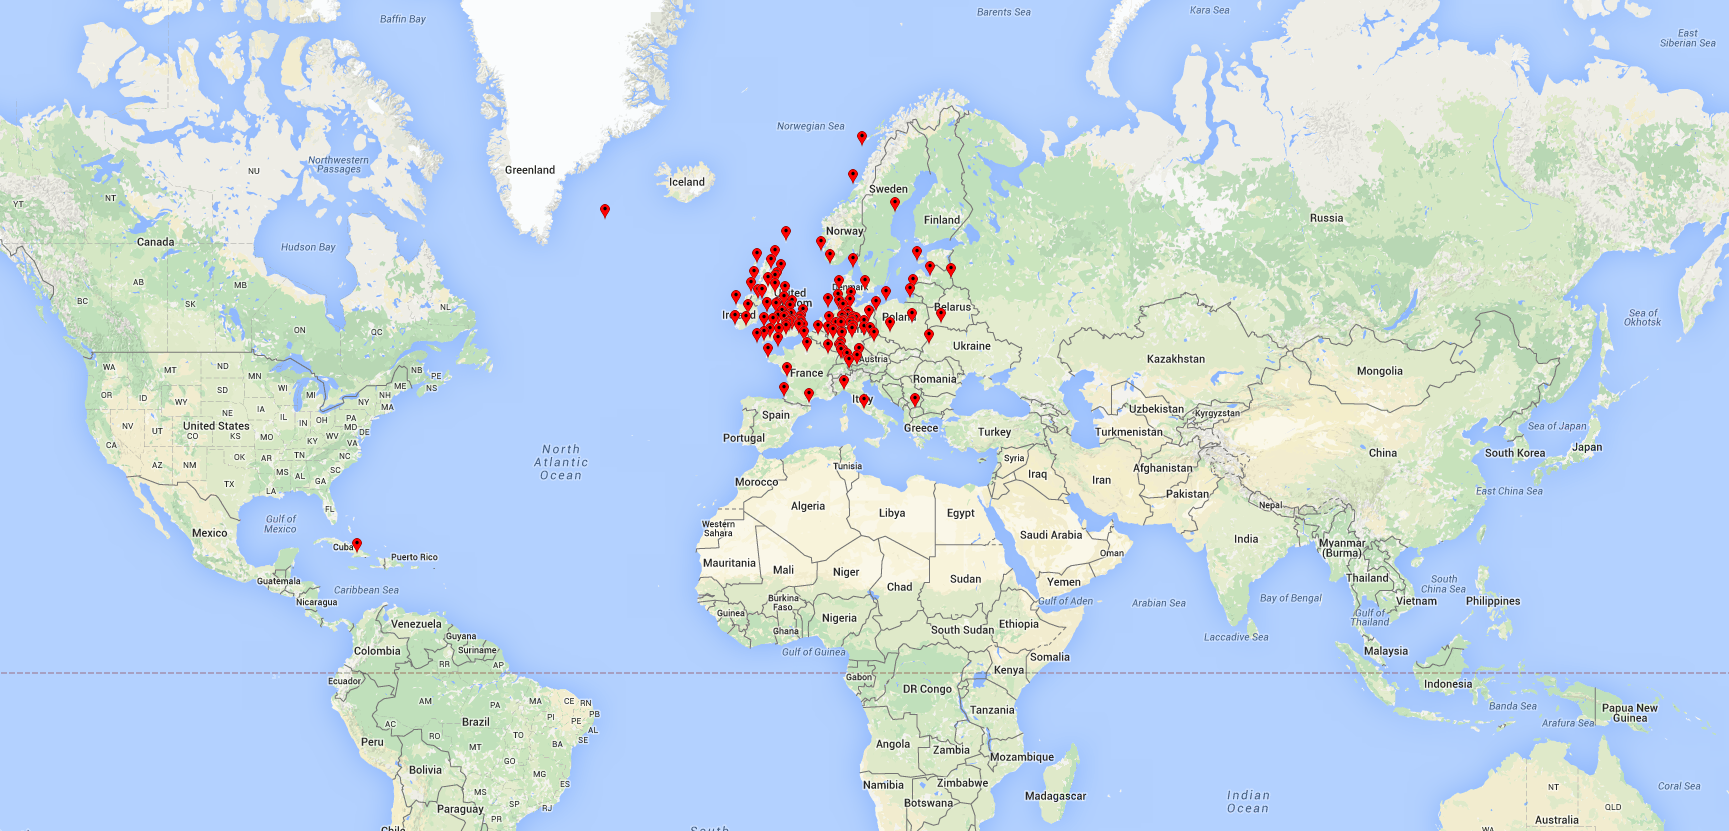
\includegraphics[width=1\linewidth]{stations1930}
\caption{Weather stations used in 1930. Here we can see the stations cover the most part of central Europe. The problem we encountered is that there is no continuity in the stations that are used between consecutive years, so it's difficult to make comparisons.}
\label{fig:stations1930}
\end{figure}

\begin{figure}[tbh]
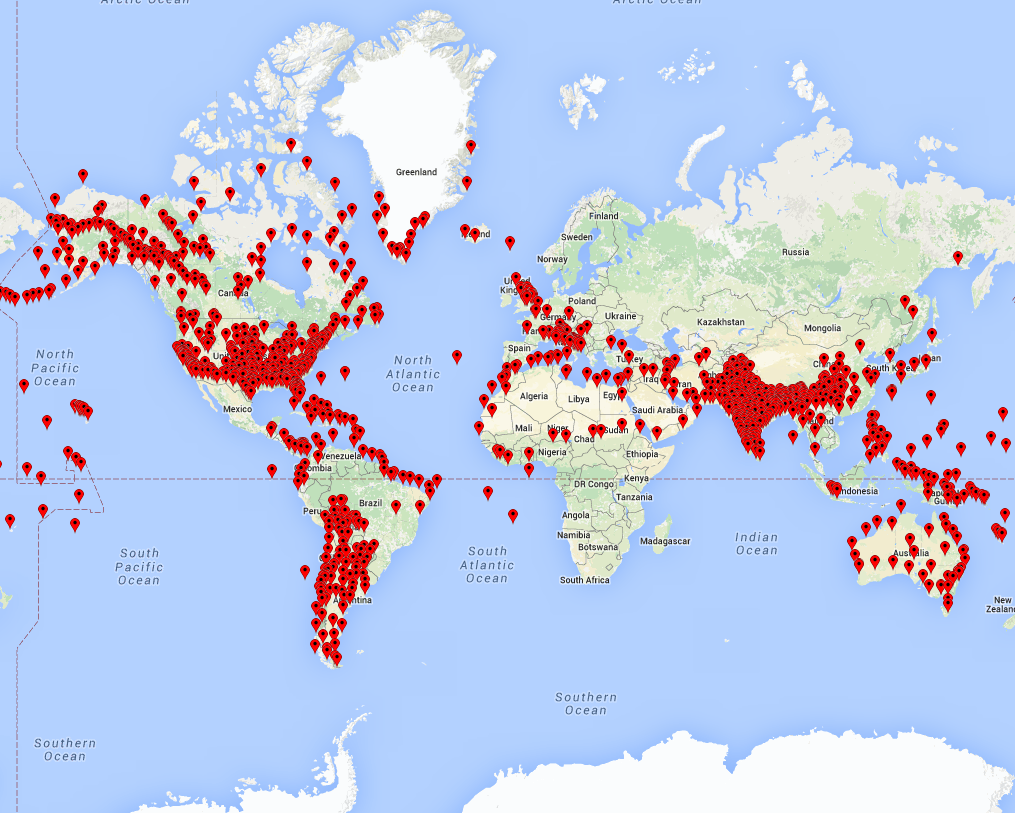
\includegraphics[width=1\linewidth]{stations1945}
\caption{Weather stations used in 1945. Around this year we start to have a relevant number of stations that cover most part of the surface.}
\label{fig:stations1945}
\end{figure}

\begin{figure}[tbh]
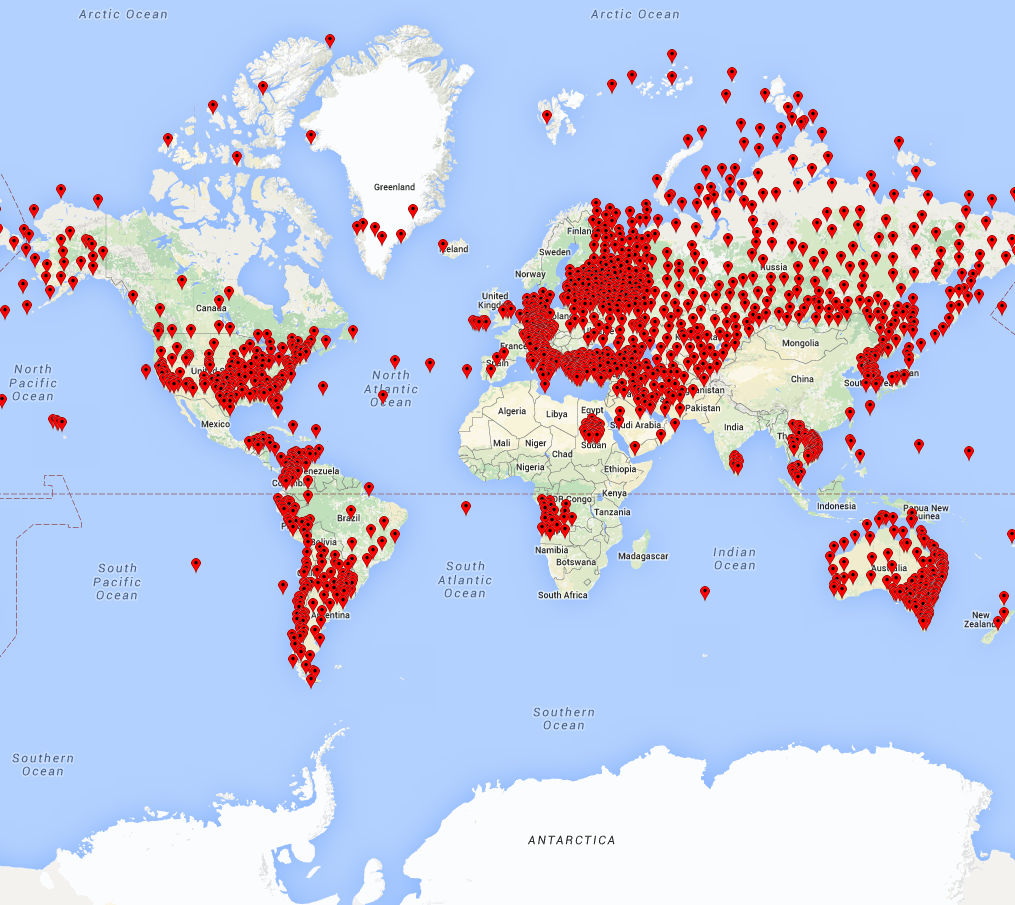
\includegraphics[width=1\linewidth]{stations1968}
\caption{Weather stations used in 1968. In the late 60s we notice a sudden drop in the earth coverage compared to the previous years. We took this into account when making the analysis.}
\label{fig:stations1968}
\end{figure}

\begin{figure}[tbh]
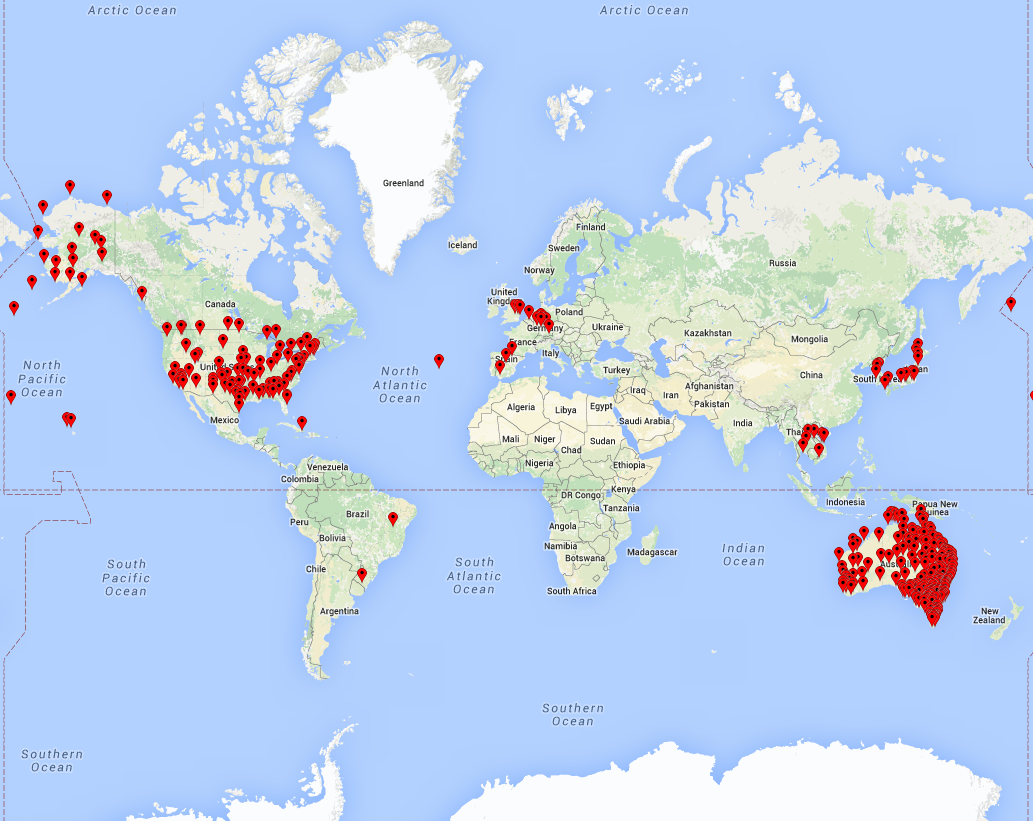
\includegraphics[width=1\linewidth]{stations1972}
\caption{Weather stations used in 1972. As shown in figure \ref{fig:stations}, we noticed a sudden drop in the number of stations for this year. In particular we observe the absence of stations from east Europe and the ex Soviet Union Area.}
\label{fig:stations1972}
\end{figure}

\begin{figure}[tbh]
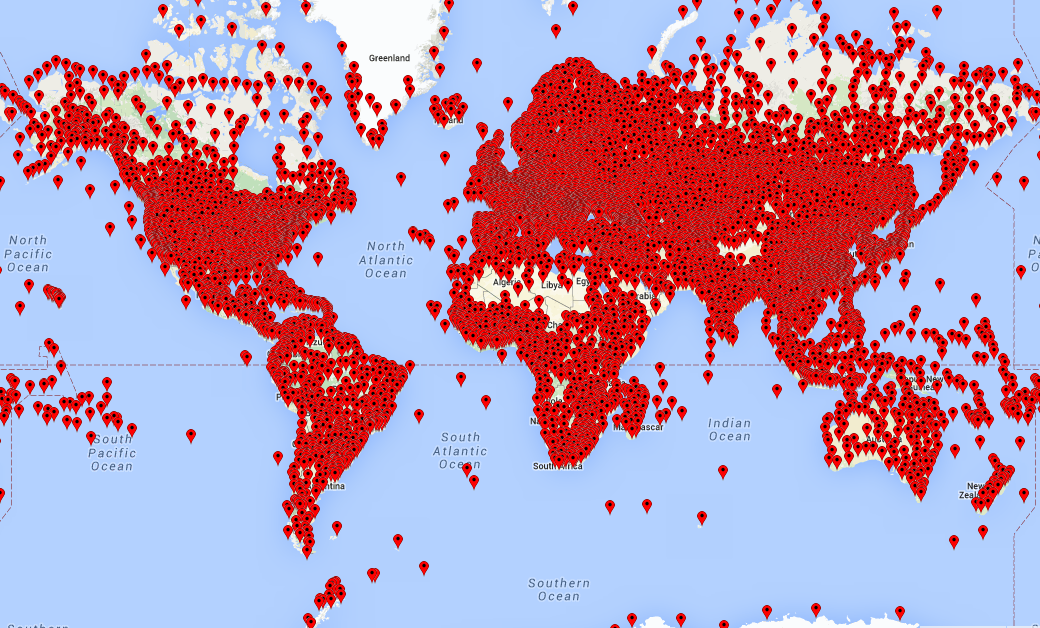
\includegraphics[width=1\linewidth]{stations1980}
\caption{Weather stations used in 1980. From this year onwards we have a large number of stations covering most part of the surface.}
\label{fig:stations1980}
\end{figure}

\begin{figure}[tbh]
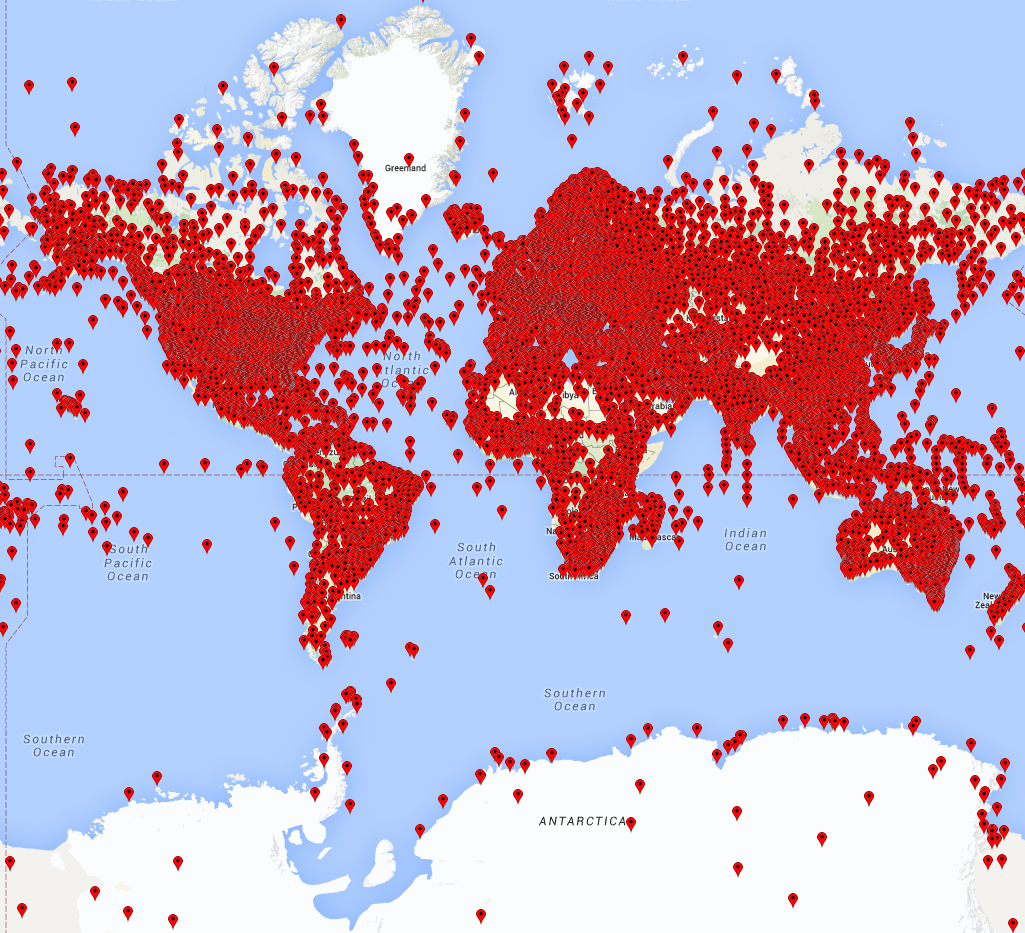
\includegraphics[width=1\linewidth]{stations2014}
\caption{Weather stations used in 2014.}
\label{fig:stations2014}
\end{figure}


\FloatBarrier
\clearpage
%\end{document}  % This is where a 'short' article might terminate

% ensure same length columns on last page (might need two sub-sequent latex runs)

%ACKNOWLEDGMENTS are optional
%\section{Acknowledgments}


% The following two commands are all you need in the
% initial runs of your .tex file to
% produce the bibliography for the citations in your paper.
% You must have a proper ".bib" file
%  and remember to run:
% latex bibtex latex latex
% to resolve all references

%Generated by bibtex from your ~.bib file.  Run latex,
%then bibtex, then latex twice (to resolve references).
\balance
\printbibliography


\end{document}
